% Introduction
\section{Introduction}\label{introduction}
	Route planning refers to the problem of finding an \textit{optimal} route between given locations in a network.
	With the ongoing expansion of road and public transit networks all over the world route planner gain more and
	more importance. This led to a rapid increase in research \libref{routePlanningOverview, networks, transitModels}
	of relevant topics and development of route planner software \libref{navHistoryEarly, navHistoryNewer, vehicleNavigation}.
	
	However, a common problem of most such services is that they are limited to one transportation mode only.
	That is a route can only be taken by a car or train but not by both at the same time. This is known as \uniModal routing.
	In contrast to that \multiModal routing allows the alternation of transportation modes. For example a route that
	first uses a car to drive to a train station, then a train which travels to a another train station and finally
	using a bicycle from there to reach the destination.
	
	The difficulty with \multiModal routing lies in most algorithms being fitted to networks with specific properties.
	Unfortunately, road networks differ a lot from public transit networks. As such, a route planning algorithm
	fitted to a certain type of network will likely yield undesired results, have an impractical running time or not
	even be able to be used at all on different networks. We will explore this later in \sectionref{evaluation}.\\\\
	In this thesis we explore a technique with which we can combine an algorithm fitted for road networks with an algorithm
	for public transit networks. Effectively obtaining a generic algorithm that is able to compute routes on combined networks.
	The basic idea is simple, given a source and destination, both in the road network, we select \textit{access nodes} for both.
	This are nodes where we will switch from the road into the public transit network. A route can then be computed by
	using the road algorithm for the source to its access nodes, the transit algorithm for the access nodes of the source
	to the access nodes of the destination and finally the road algorithm again for the destinations access nodes to
	the destination. Note that this technique might not yield the shortest possible path anymore. Also, it does not allow
	an arbitrary alternation of transportation modes. However, we accept those limitations since the resulting
	algorithm is very generic and able to compute routes faster than without limitations. We will cover this technique in detail
	in \sectionref{accessNodes}.\\\\
	Our final technique uses a modified version of \alt \libref{alt} as road algorithm and \csa \libref{csa} for the transportation network.
	The algorithms are presented in \sectionref{alt} and \sectionref{csa} respectively.
	We also develop a \multiModal variant of \dijkstra \libref{dijkstra} which is able to compute the shortest route in a combined
	network with the possibility of changing transportation modes arbitrarily. It is presented in \sectionref{modifiedDijkstra}
	and acts as baseline to our final technique based on access nodes.
	
	We compute access nodes by solving the \nearestNeighborProblem. For a given node in the road network its access
	nodes are then all nodes in the transit network which are in the \textit{vicinity} of the road node. We explore a solution
	to this problem in \sectionref{nearestNeighborProblem}.\\\\
	\sectionref{models} starts by defining types of networks. We represent road networks by graphs only.
	For transit networks we provide a graph representation too. Both graphs can then be combined into a linked graph.
	The advantage of graph based models is that they are well studied and therefore we are able to use our
	\multiModal variant of \dijkstra to compute routes on them.
	However, we also propose a non-graph based representation for transit networks, a timetable. The timetable is used by \csa,
	an efficient algorithm for route planning on public transit networks. With that, our road and transit networks get incompatible
	and can not easily be combined. Therefore, we use the previously mentioned generic approach based on access nodes
	for this type of network.\\\\
	% Cobweb frontend screenshot
	\begin{figure}[!ht]
		 \begin{center}
			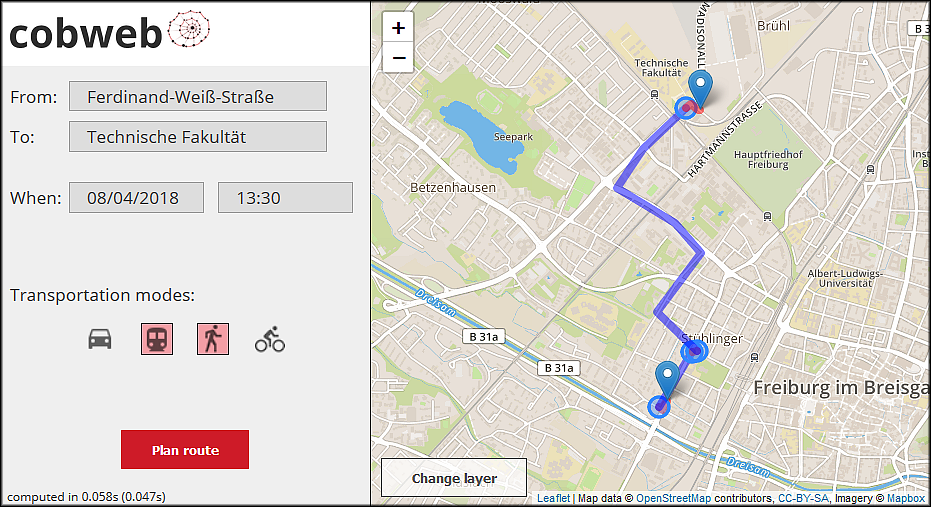
\includegraphics[scale=0.5]{res/cobweb_frontend}
		\end{center}
		\caption{Screenshot of {\cobweb}s \libref{cobweb} frontend, an open-source \multiModal route planner. It shows a \multiModal
		route starting from a given source, using the modes \textit{foot-tram-foot-tram-foot} in that sequence to reach the destination.}
		\label{cobweb_frontend}
	\end{figure}\quad\\
	Further, we implemented the presented algorithms in the \cobweb \libref{cobweb} project, which is an open-source \multiModal
	route planner (see \figref{cobweb_frontend} for an image of its frontend).
	In \sectionref{evaluation} we show our experimental results and compare the techniques with each other.